\kap{In-Medium Scattering}\label{chap:In-Medium Scattering} 
So far only free NN scattering has been considered. From this data there have built different potential
like the nna13 potential, which is fairly good up to 1 GeV. Since the strong force is a three body force, we will
experience different potential between two free nucleons than two nucleons in a nuclear with three or more nucleons. 
However, most of the many-body theory today is based on the potential made from simple NN-systems.

The spherical geometry and the boundary conditions 
of the nuclears, makes it difficult to make a mathematical model of the situation. A commonly used 
simplification to the problem, is to introduce
the theoretical "nuclear matter"-model. This model is very similar to the situation inside heavy nuclears.
In order to describe the situation one also have to include properties from many particle theory 
like the Pauli effect and the dispersion effect.
\section{Nuclear Matter}
Nuclear matter is from definition  a infinite system nucleons, which are only interacting through the strong force,
i.e. all the other forces are neglected. This situation is an approximation to the real situation we
have in heavy nuclears. Nucleons in the boundary of the nuclear will behave slightly different, 
and the approximation will be better the closer the nucleon are to the center of the heavy nuclear.
A nice mathematical property of the nuclear matter model is that such a system is translation invariant.

The non relativistic Hamiltonian of an interacting many-particle system is
\begin{eqnarray}\label{eq:first-quant}
\op{H}&=&\op{T}+\op{W}+\op{V}\nonumber\\
      &=&\sum^N_{i=1}\frac{{{{\bf p}}}^2_i}{2m}+\sum^N_{i=1}w({{\bf r}}_i)+\sum^N_{i<j}v({{\bf r}}_i,{{\bf r}}_j)
\end{eqnarray}
Where $N$ is the number of particles in the system. For a translational system we must have
\begin{equation}
w({{\bf r}})={\text{constant}}
\end{equation}
This is precisely what we achieve in creating a uniform system like the nuclear matter model. Where the
potential from the nucleons position in the nuclear matter is the same for all the nucleons because there are no boundary effects 
in this model, and the nuclear matter is symmetric. If we also assume that there are non external potential to the system,
we have $w({{\bf r}})=0$

In the nuclear matter model the single particle waves can be expressed in plane waves instead of self-consistent Hartree-Fock wave
functions we get from solving the exact problem with heavy nuclears.
The eigenfunction of plane waves are
\begin{equation}
\phi_{{\bf {k}}\sigma}(x)=\frac{1}{\sqrt{\Omega}}e^{i{\bf {kr}}}\chi_\sigma(s)
\end{equation}
Where $\sigma(s)$ denotes the usual Pauli-spinor and $\Omega$ is the volume element we need to normalize the wave function.
In second quantization \ref{eq:first-quant} can be rewritten
as
\begin{eqnarray}\label{eq:seceond-quant}
\op{H}&=&\sum_{{{\bf {k}}\sigma}}\bigg(\frac{{\bf {k}}^2}{2m}+w\bigg)
\op{c}^\dagger_{{{\bf {k}}\sigma}}\op{c}_{{{\bf {k}}\sigma}}
\nonumber\\
      &&+\frac{1}{2\Omega}\sum_{{\bf {q}}}\sum_{{{\bf {k}}\sigma},{{\bf {k}}'\sigma'}}
      v_{{\bf {q}}}
      \op{c}^\dagger_{({{\bf {k}}+{{\bf {q}}})\sigma}}\op{c}^\dagger_{({{\bf {k}}'-{{\bf {q}}})\sigma'}}
      \op{c}_{{{\bf {k}}'\sigma'}} \op{c}_{{{\bf {k}}\sigma}} 
\end{eqnarray}

To get the nuclear matter model as close to the real situation in the interior of a heavy nuclear, the nuclear matter density
is chosen to be the same as the observed one in heavy nuclears.
\begin{equation}
\rho=0.17\pm 0.02\quad {\text fm}^{-3}
\end{equation}
The Fermi momentum $k_F$ can be defined as
\begin{equation}
k^3_F=\frac{3}{2}\rho\pi^2
\end{equation}
From these two equations we have
\begin{equation}
k_F=1.35\pm0.05\quad {\text fm}^{-1}
\end{equation}
The Fermi momentum is an important factor in the phase shift analysis, which arrives from the Pauli effect in medium.









\section{Many-body Theory}
The theory dealt with here is constructed from the wish of explaining the the interactions through a
two-body potential. So that we can use the potential from the NN interaction to explain all the different nucleon configurations, 
or that is at least the ultimate goal of the theory.

The perturbation theory is developed around the Hartree-Fock approximation, where the unperturbated Hamiltonian $H_{\text{HF}}$
is the effective single particle Hamiltonian. Eq(\ref{eq:first-quant}) can then be written as
\begin{eqnarray}\label{eq:HF-approx}
\op{H}&=&\sum^N_{i=1}\bigg( \op{t}_i+\op{u}_i\bigg)+\bigg(\sum^N_{i<j}\op{v}_{ij}-\sum^N_{i=1}\op{u}_i\bigg) \nonumber\\   
      &=&\op{H}_{\text{HF}}+\op{H}'
\end{eqnarray}
Where the external potential is neglected. $\op{H}'$ is the perturbation.
Since the nucleons are Fermions, one have to use Slater determinants of single-particle orbitals as a basis for
the total many body wave function. These Slater determinants should also include the Pauli spinor, so that 
spin properties of the system is accounted for.
This way the Hamiltonian ${\op{H}}$ will commute with the square and the z-component 
of the total angular momentum and total spin. 
One can calculate the expectation value of $\op{H}$ with a Slater determinant basis (${{ \Phi}}$). Here written in second quantization
\begin{equation}\label{eq:HF-sec} 
\braketm{{{ \Phi}}}{\op{H}}{{{ \Phi}}}
=\sum^N_{i=1}\braketm{i}{h_{HF}}{i}+\frac{1}{2}\bigg(\sum^N_{i,j=1}\braketm{ij}{v}{ij}-\sum^N_{i,j=1}\braketm{ij}{v}{ji}\bigg) 
\end{equation}
We see that the interaction potential consists of two terms. It has been normal to call
the first term in the brackets in (\ref{eq:HF-sec}) for the direct term. The second is called the exchange term.
UFERDIG!!!!!!!!!!!!!!!





\section{Minimal Relativity With Build-In Dispersion Effect}
The Minimal relativity equation in free space is
\begin{equation}\label{eq:Trelllllfree}
\braketm{{ p}} {\op{T}_l(E_{ k})}{{ k}}=\braketm{{ p}}{\op{V}_l}{{ k}}
+ \frac{2}{\pi}%\;{\cal P}
\int^{\infty}_{0}d { q}\; q^2\bra{{ p}}\op{V}_l\ket{{ q}}
\;\inv{{\varepsilon(k)}-{\varepsilon(q)\pm i\epsilon}}   \;\bra{{ q}} \op{T}_l(E_{ k})\ket{{ k}}
%\nonumber\\
%&&
%-i { k}m \bra{{ p}}\op{V_l}\ket{{ k}}
%\;\bra{{ k}}\op{T}_l(E_{ k})\;\ket{{ k}}
\end{equation}
where $\varepsilon(k)$ is the free two nucleons energy in the center of mass 
\begin{eqnarray}
\varepsilon(k)=\frac{k^2}{m_{{\text N}}}+m_{{\text N}}
\end{eqnarray}
In a medium this energy can be written as a dispersion relation, where the energy is a function of the momentum
\begin{eqnarray}\label{eq:inmediumeps}
\widetilde{\varepsilon}(k)=\frac{k^2}{m_{{\text N}}}+m_{{\text N}}+U(k)
\end{eqnarray}
The potential $U(k)$ arises because the nucleons interact with the nuclear matter. This potential will be negative
for small k (i.e feels an attractive force from the nucleons in the nuclear matter. The potential
is found to be on the form  
\begin{eqnarray}
U(k)\approx {{\text c}}k^2-U_0
\end{eqnarray}
Where c is a constant.
With this approximation we can rewrite  (\ref{eq:inmediumeps}).
\begin{eqnarray}\label{eq:inmediumeps2}
\widetilde{\varepsilon}(k)=\frac{k^2}{m^*_{{\text N}}}+m_{{\text N}}-U_0
\end{eqnarray}
The effective mass $m^*$ is a commonly used in many particle models. In nuclear matter it is found
to be about 688 MeV. This is done by using Brecner theory, where one first guess a $m^*_{{\text N}}$ to use. 
From the theory one can then calculate a better $m^*_{{\text N}}$, which one use again and again until self consistent is achieved.
More about this both relativistic and non relativistic are explained in~\cite{Macbok}.
The propagator term in the $\LS$ equation will be dependent on the difference of $\widetilde{\varepsilon}(k)$ 
and $\widetilde{\varepsilon}(q)$. This effect is called "Dispersion effect" 
\begin{eqnarray}\label{eq:inmediumeps3}
\widetilde{\varepsilon}(k)-\widetilde{\varepsilon}(q)=\frac{k^2}{m^*_{{\text N}}}-\frac{q^2}{m^*_{{\text N}}}
\end{eqnarray}
The new $\LS$ equation with this Dispersion effect included, will be
\begin{eqnarray}\label{eq:Trelllllnoererw}
\braketm{{ p}} {\op{T}_l(E_{ k})}{{ k}}&=&\braketm{{ p}}{\op{V}_l}{{ k}}
+ \frac{2m^*_{{\text N}}}{\pi}\;{\cal P}\int^{\infty}_{0}d { q}\; q^2 \quad\bra{{ p}}\op{V}_l\ket{{ q}}
\;\inv{{ k^2}-{ q^2}}   \;\bra{{ q}} \op{T}_l(E_{ k})\;\ket{{ k}}\nonumber\\
&&
-i { k}m^*_{{\text N}} \bra{{ p}}\op{V_l}\ket{{ k}}
\;\bra{{ k}}\op{T}_l(E_{ k})\;\ket{{ k}}
\end{eqnarray}
For the relation between the on-shell momentum k in the center of mass system and the lab energy $T_{{\text lab}}$
is the same as before. Namely,
\begin{eqnarray}
k=\sqrt{\frac{m_{{\text N}}T_{{\text lab}}}{2}}
\end{eqnarray}
Where m is again the free mass of a nucleon.




\section{The Pauli Effect in nuclear matter}
The Pauli effect is a direct consequence of the Pauli principal and the model we use to describe the nuclear matter.
If we assume that all the nucleons in the nuclear matter are in the lowest eigen states possible, and we name
the state whit the highest energy to be the Fermi momentum $k_{{\text F}}$. Because of the
Pauli principal, all the interacting nucleons have to be in different energy states. If the energy states up till
$k_{{\text F}}$ are occupied by the nucleons in the nuclear matter, the allowed energy states for
the nucleons being scattered have all $k\ge k_{{\text F}}$. In operator form we include the Pauli operator $Q$
in the propagator in the $\LS$ equation from   (\ref{eq:TM}) 
\begin{equation}\label{eq:TM22222}
\op{T}=\op{V}+\op{V}Q\op{G}^{}_0\op{T}
\end{equation}
The Pauli operator $Q$ projects only onto the unoccupied states. In partial wave decomposition in
momentum space this will be
\begin{equation}\label{eq:Trelllllinmed}
\braketm{{ p}} {\op{T}_l(E_{ k})}{{ k}}=\braketm{{ p}}{\op{V}_l}{{ k}}
+ \frac{2m^*_{{\text N}}}{\pi}%\;{\cal P}
\int^{\infty}_{k_{{\text F}}}d { q}\; q^2\bra{{ p}}\op{V}_l\ket{{ q}}
\;\inv{{k^2}-q^2\pm i\epsilon}   \;\bra{{ q}} \op{T}_l(E_{ k})\ket{{ k}}
%\nonumber\\
%&&
%-i { k}m \bra{{ p}}\op{V_l}\ket{{ k}}
%\;\bra{{ k}}\op{T}_l(E_{ k})\;\ket{{ k}}
\end{equation}
Where also the dispersion effect has been included.





\section{Dispersion Effect involving $\triangle$-excitations} 
The next step will be to include the effective mass of the nucleons in the
$\triangle$-excitations diagrams. By including the in-medium effect in the one $\triangle$-excitation
propagator $\widetilde{\epsilon}_\triangle$ in the coubled channel equation. 
\begin{equation}\label{eq:TM22222344444444}
\frac{1}{\widetilde{\epsilon}_{{\text N}}({{ k}})+
\widetilde{\epsilon}_\triangle({{ k}})-2\widetilde{\epsilon}_{{\text N}}({{ k}}_0)}
\end{equation}
Where $\widetilde{\epsilon}_{{\text N}}({{ k}}_0)$ is the total energy in the center of mass system.
The two $\triangle$-excitation if included should also be changed in the same way.
If we neglect the in-medium effect on the $\triangle$ particles, which was also done for the mesons
\begin{equation}
\widetilde{\epsilon}_\triangle={\epsilon}_\triangle=\frac{{{ k}}^2}{2m_\triangle}+(m_\triangle-m_{{\text N}})  
\end{equation} 
Where ${\cal R}{e}[m_\triangle]=1232$ MeV. The in medium effect on the propagator in (\ref{eq:TM22222344444444})
is therefor only in the $\widetilde{\epsilon}_{{\text N}}({{ k}})$ part, which is given in
(\ref{eq:inmediumeps2}).

This in-medium effect has been built in to the potential nna13 and this version is called nna13in. 





\section{Numerical Solution Of In Matter Scattering}

The Dispersion effect is included in the computer program if all the Nucleon masses ($m=m_{{\text N}}$) 
are changed to the effective mass ($m^*=m^*_{{\text N}}$), except in the calculation of the on-shell momentum in
the center of system $k({{\text N}}+1)$.

The Pauli effect is included by changing the integral from $(0,\infty) \to (k_{{\text F}},\infty)$.
Numerically this can be done by adding $k_{{\text F}}$ to all the mesh points (not to $k({{\text N}}+1)$),i.e.
\begin{equation}\label{eq:TM2222233333}
q_i=q_i+k_{{\text F}},\qquad {{\text for}}\quad i\le N
\end{equation}
Where N is the number of mesh points.
By changing the integral limits, we also change the limits on the term that numerically removes the singularity
in the integrand (\ref{eq:trix0}). 
\begin{equation}\label{eq:trix022222}
-\frac{2m^*}{\pi}\;k^2\bra{{ p}}\op{V}_l\ket{{ k}}
\bra{{ k}} \op{T}_l\;\ket{{ k}}\;{\cal }\int^{\infty}_{k_{{\text F}}}\frac{d q}{k^2-{ q^2}}\neq0
\end{equation}
This term is no longer zero, and one can therefor not add this
equation to ( \ref{eq:Trelllllinmed}). However if we also add
\begin{equation}\label{eq:trix02222233}
-\frac{2m^*}{\pi}\;k^2\bra{{ p}}\op{V}_l\ket{{ k}}
\bra{{ k}} \op{T}_l\;\ket{{ k}}\;{\cal }\int^{k_{{\text F}}}_{0}\frac{d q}{k^2-{ q^2}}
\end{equation}
to  (\ref{eq:trix022222}) the two terms will together be zero. Equation (\ref{eq:trix02222233})
can be calculated analytically:
\begin{equation}\label{eq:trix0222223344}
-\frac{2m^*}{\pi}\;k^2\bra{{ p}}\op{V}_l\ket{{ k}}
\bra{{ k}} \op{T}_l\ket{{ k}}\;{\cal }\int^{k_{{\text F}}}_{0}\frac{d q}{k^2-{ q^2}}
=
-\frac{m^*k}{\pi}\bra{{ p}}\op{V}_l\ket{{ k}}
\bra{{ k}} \op{T}_l\ket{{ k}}
\log\bigg|\frac{k_{{\text F}}+k}{k_{{\text F}}-k}\bigg|
\end{equation}
The numerical equations we get from (\ref{eq:trix022222}) is therefor
\begin{eqnarray}\label{eq:Trelllllaae22222222}
\braketm{{ p}}{\op{V}_l}{{ k}}&=&\braketm{{ p}} {\op{T}_l}{{ k}}
- \frac{2m^*}{\pi}\sum^N_{j=1}
\frac{\omega_j q^2_j}{{ k^2}-{ q^2_j}}\bra{{ p}}\op{V}_l\ket{{ q_j}} \bra{{ q_j}} \op{T}_l\ket{{ k}}\nonumber\\
&&+
\frac{2m^*}{\pi}\bra{{ p}}\op{V}_l\ket{{ k}}
\bra{{ k}} \op{T}_l\ket{{ k}}\sum^N_{j=1} \frac{\omega_jk^2}{{ k^2}-{ q^2_j}}\nonumber\\
&&-
m^*k\bigg(i+\frac{1}{\pi}\log\bigg|\frac{k_{{\text F}}+k}{k_{{\text F}}-k}\bigg|\bigg)
\bra{{ p}}\op{V_l}\ket{{ k}}
\bra{{ k}}\op{T}_l\ket{{ k}}
\end{eqnarray}
Comparing this equation with (\ref{eq:Trelllllaae}) we see that this will only change
the $u({{\text N}}+1)$ matrix given in (\ref{eq:ujN1}). The $u(q_i)$ elements will be the same as before and the 
new $u({{\text N}}+1)$ matrix element will be
\begin{equation}\label{eq:ujN1222}
u_{N+1}=-\frac{2m^*}{\pi}\sum^N_{j=1}\frac{\omega_jq^2_{N+1}}{{ q^2_{N+1}}-{ q^2_j}}+  im^* q_{N+1}
+\frac{m^*q_{N+1}}{\pi}\log\bigg|\frac{k_{{\text F}}+q_{N+1}}{k_{{\text F}}-q_{N+1}}\bigg| 
\end{equation}
The Thompson method will be similar.





\section{Results}
The inmedium effects that are included are the Pauli effect and the effect from the dispersion relation.
The latest effect are included for OBE and/or  $\triangle$ and $\triangle\triangle$ excitation diagrams.
These results from the in-medium scattering calculations are plotted together with the free
case in (\ref{figInmediumphaseSandI}) and 
(\ref{figInmediumCrossS})

The next effects to include in this model will be effects like the interaction between the mesons and
the nuclear matter, and more important the Dirac effect. The Dirac effect is derived by using the Dirac-Bruckner
approach and let the effective mass enter the picture already Dirac spinors from the solution of the Dirac equation.
This relativistic potential is different from the non relativistic potential. More about Dirac-Bruckner approach
in (\cite{In-med-DiracBruck}).
\nl
Fig(\ref{figInmediumCrossS}) shows how important it is to include the dispersion relation also in the
$\triangle$ propagator.



\begin{figure}
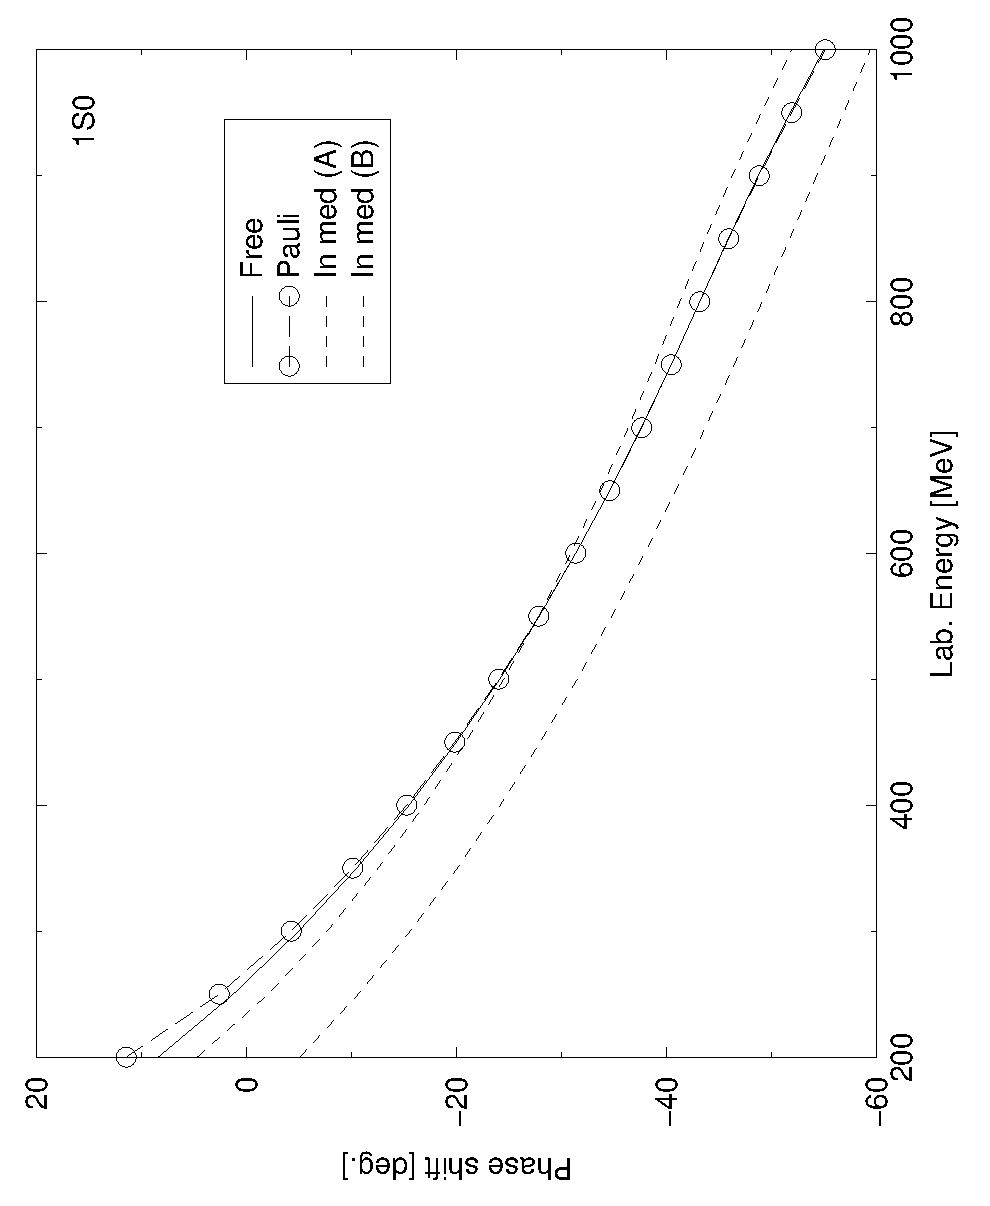
\includegraphics[height=7cm,width=7cm,angle=-90]{iii_elastinmedium.eps}
\qquad
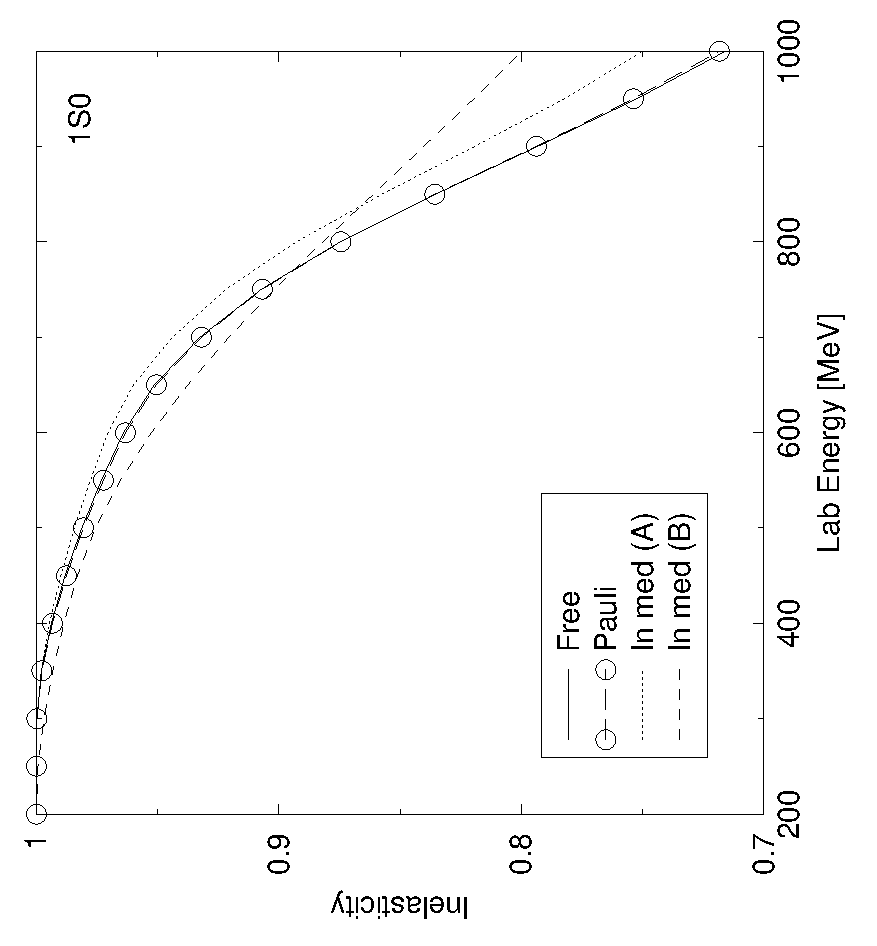
\includegraphics[height=7cm,width=7cm,angle=-90]{inelastinmedium.eps}
\caption{
\label{figInmediumphaseSandI}
Free and in-medium np scattering phase shifts and inelasticities for the partial \state{1}{S}{0}-state. 
as a function of of the incident energy. Where the free np scattering,
and three In-medium cross sections have been plotted. "Pauli" has only been included
the Pauli effect. "In med (A)" have only been included in-medium effects in the
$\LS$ equation. "In med (B)" has also been included the in-medium $\triangle$ effect. The results are obtained from 
the nna13 potential.
}
\end{figure}
\begin{figure}
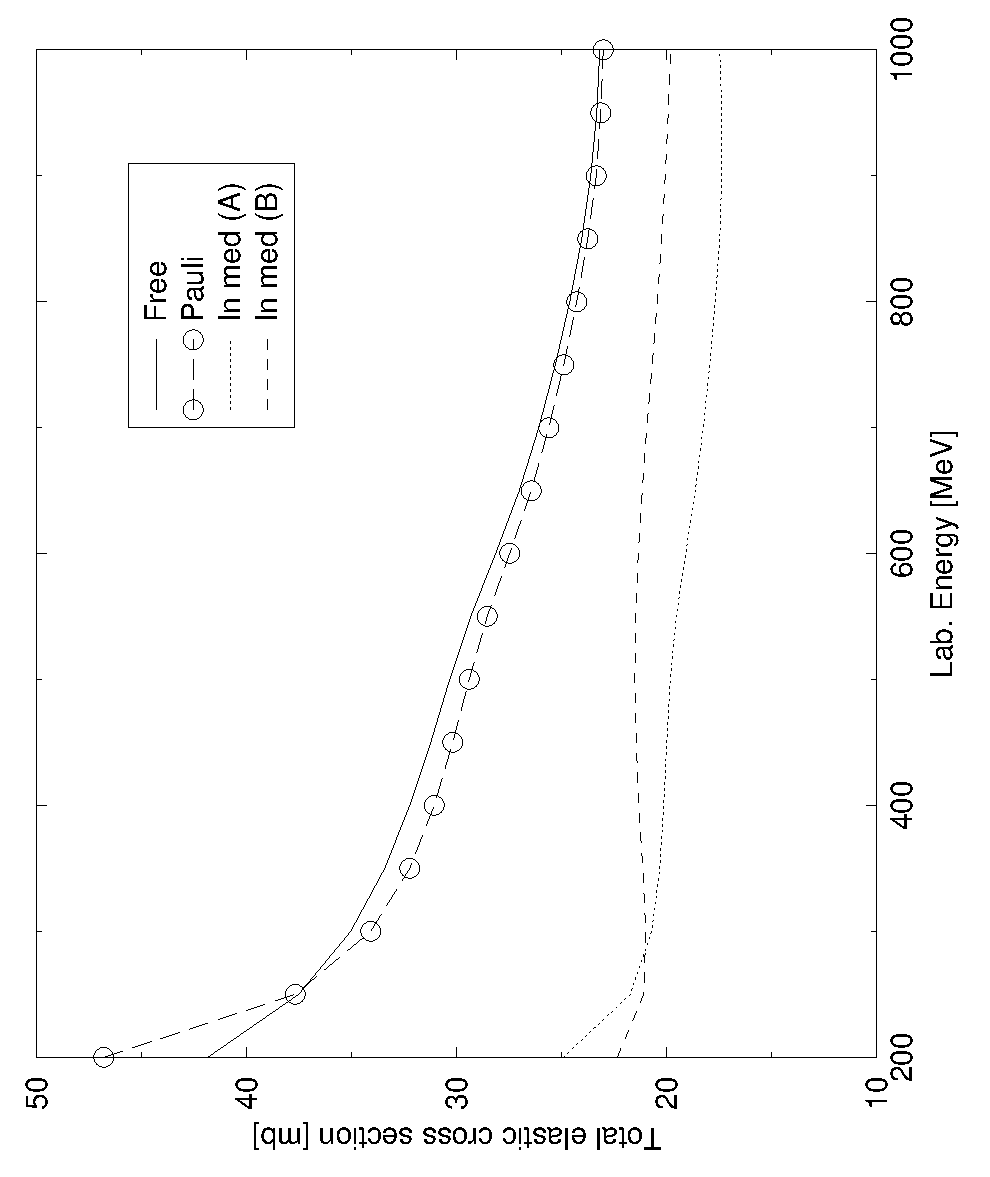
\includegraphics[height=7cm,width=7cm,angle=-90]{iii_crossPhaseS.eps}
\qquad
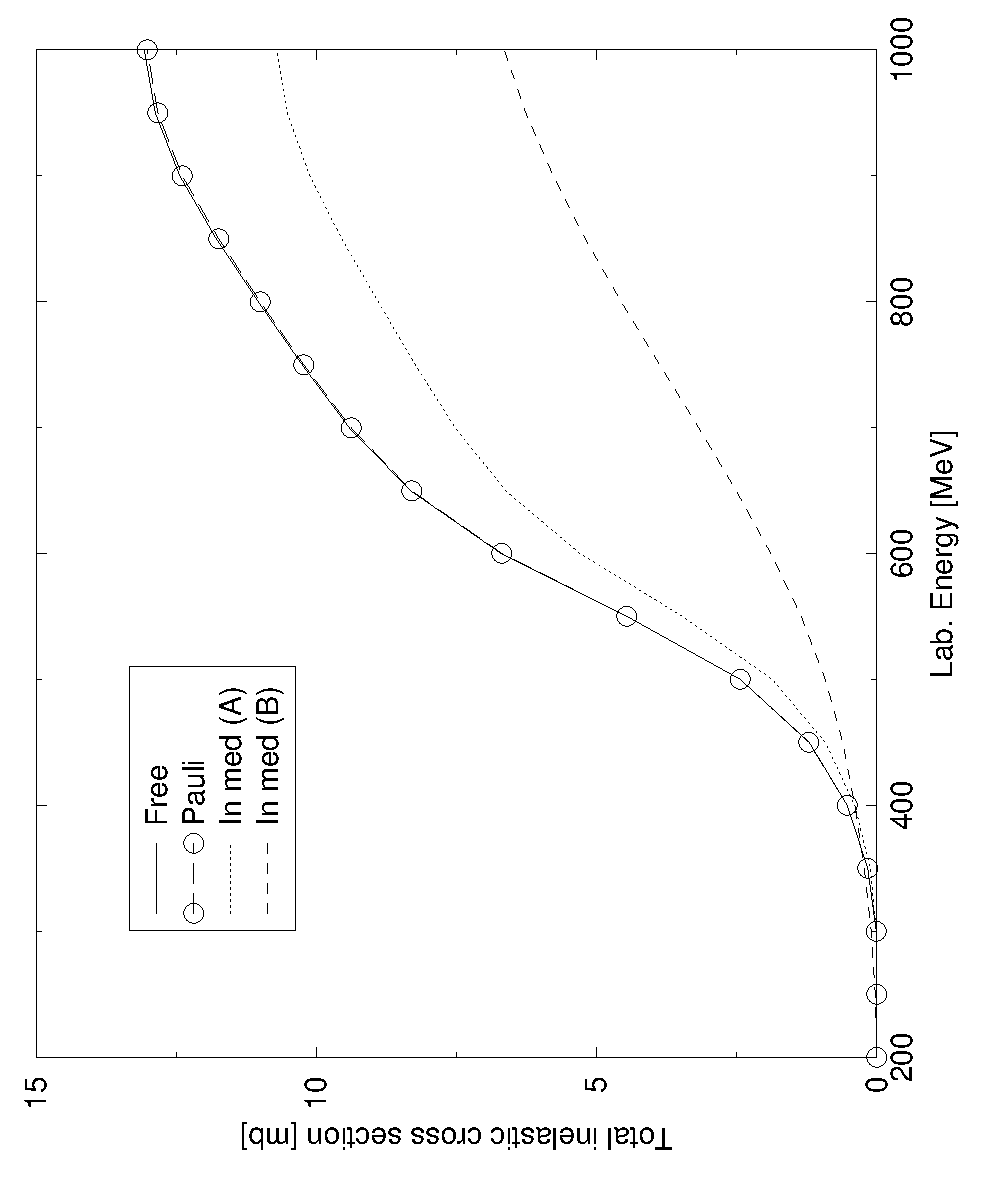
\includegraphics[height=7cm,width=7cm,angle=-90]{iii_crossInEl.eps}
\caption{
\label{figInmediumCrossS}
Free and in-medium np scattering cross sections.
Total cross sections for np scattering as a function of of the incident energy. Where the free np scattering,
and three In-medium cross sections have been plotted."Pauli" has only been included
the Pauli effect. "In med (A)" have only been included in-medium effects in the
$\LS$ equation. "In med (B)" has also been included the in-medium $\triangle$ effect. The results are obtained from
the nna13 potential.
}
\end{figure}
